%To compile as handout, use
%pdflatex "\def\ishandout{1} \input{filename.tex}"
%Defaults to non-handout mode (with slide reveals)
\ifdefined\ishandout
  \documentclass[handout]{beamer}
\else
  \documentclass{beamer}
\fi
 
\usepackage{econ103slides} 

\date{Lecture \# 12}
\begin{document} 

%%%%%%%%%%%%%%%%%%%%%%%%%%%%%%%%%%%%%%%%

\begin{frame}[plain]
	\titlepage 
	

\end{frame} 

%%%%%%%%%%%%%%%%%%%%%%%%%%%%%%%%%%%%%%%%

\begin{frame}
\begin{center}
\Huge Continuous Distributions -- Part II
\end{center}
\end{frame}


%%%%%%%%%%%%%%%%%%%%%%%%%%%%%%%%%%%%%%%%
\begin{frame}
\Huge \begin{center}
The Most Important RV of All
\end{center}

\end{frame}
%%%%%%%%%%%%%%%%%%%%%%%%%%%%%%%%%%%%%%%%
\begin{frame}
\frametitle{Normal Random Variable}
\begin{block}{Notation: $X \sim N(\mu, \sigma^2)$}
Parameters: $\mu = E[X]$, $\sigma^2 = Var(X)$\\ Support:  $(-\infty, +\infty)$
\end{block}


\begin{block}{Probability Density Function}
	$$ f(x) = \frac{1}{\sqrt{2\pi \sigma^2}} \exp \left\{ - \frac{1}{2} \left(\frac{x - \mu}{\sigma} \right)^2 \right\}$$
\end{block}


\begin{block}{No Explicit Formula for CDF (use computer instead)}
	$$F(x_0) = \int_{-\infty}^{x_0}  \frac{1}{\sqrt{2\pi \sigma^2}} \exp \left\{ - \frac{1}{2} \left(\frac{x - \mu}{\sigma} \right)^2 \right\} \; dx$$
\end{block}
\end{frame}

%%%%%%%%%%%%%%%%%%%%%%%%%%%%%%%%%%%%%%%%


\begin{frame}
\frametitle{Normal PDF Centered at the Mean (Here $\mu = 0$, $\sigma^2 = 1$)}

\begin{figure}
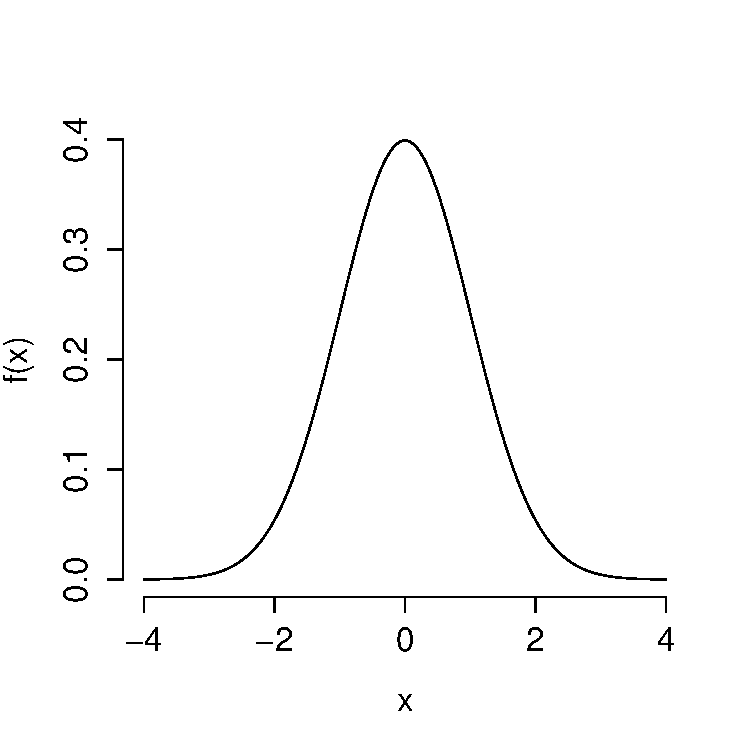
\includegraphics[scale = 0.65]{./images/std_normal_PDF}
\end{figure}
\end{frame}

%%%%%%%%%%%%%%%%%%%%%%%%%%%%%%%%%%%%%%%%



\begin{frame}
\frametitle{Normal CDF ($\mu = 0$, $\sigma^2 = 1$)}

\begin{figure}
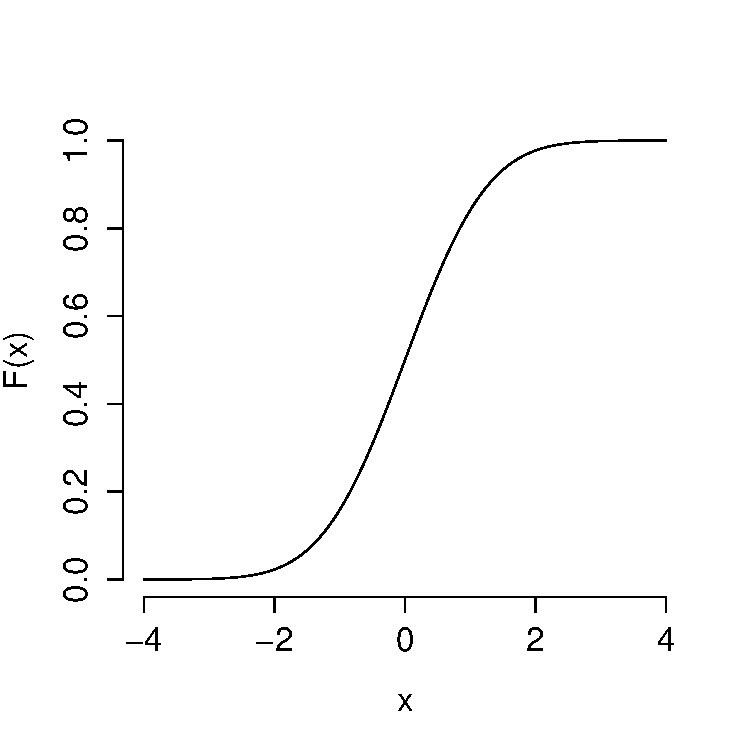
\includegraphics[scale = 0.62]{./images/std_normal_CDF}
\end{figure}
\end{frame}

%%%%%%%%%%%%%%%%%%%%%%%%%%%%%%%%%%%%%%%%

\begin{frame}
	\frametitle{\href{http://glimmer.rstudio.com/fditraglia/normal_cdf/}{http://glimmer.rstudio.com/fditraglia/normal\_cdf/}}

\begin{figure}
	\fbox{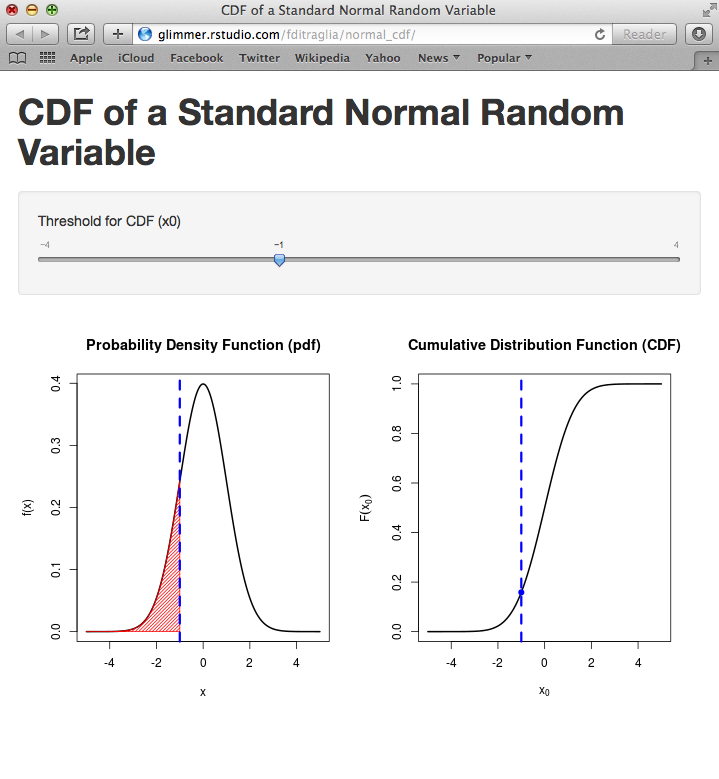
\includegraphics[scale = 0.2]{./images/normal_cdf_screenshot}}
\end{figure}

\end{frame}

%%%%%%%%%%%%%%%%%%%%%%%%%%%%%%%%%%%%%%%%




\begin{frame}
\frametitle{Different Means, Same Variance}

\begin{figure}
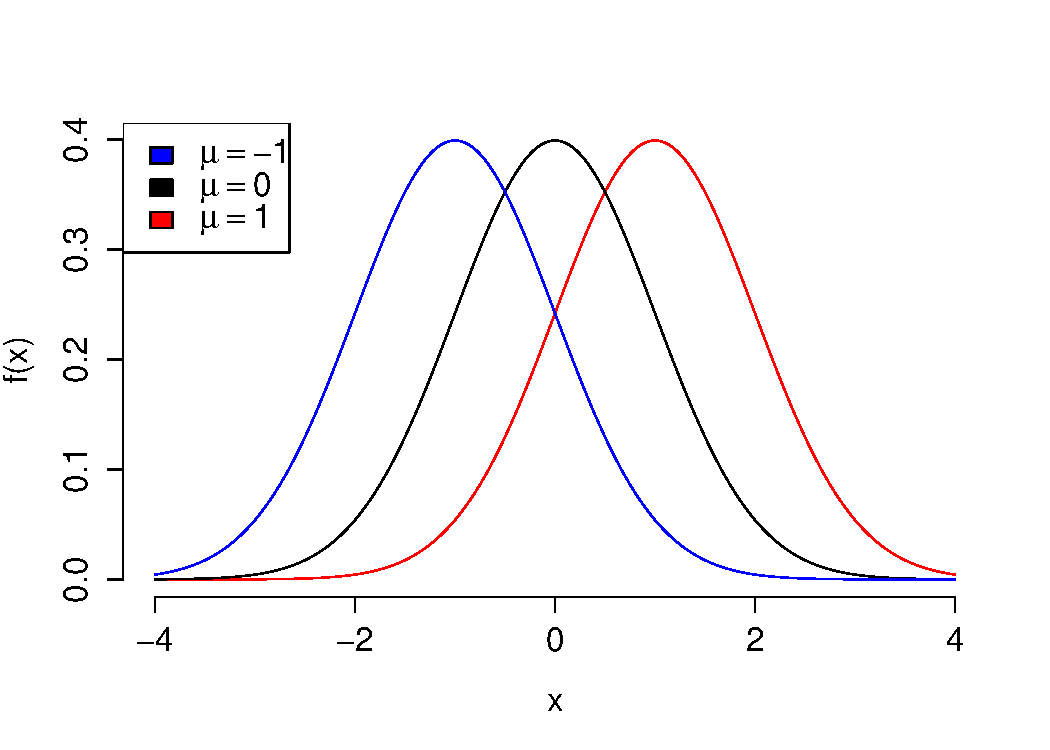
\includegraphics[scale = 0.65]{./images/normal_means}
\end{figure}
\end{frame}

%%%%%%%%%%%%%%%%%%%%%%%%%%%%%%%%%%%%%%%%


\begin{frame}
\frametitle{Same Mean, Different Variances}

\begin{figure}
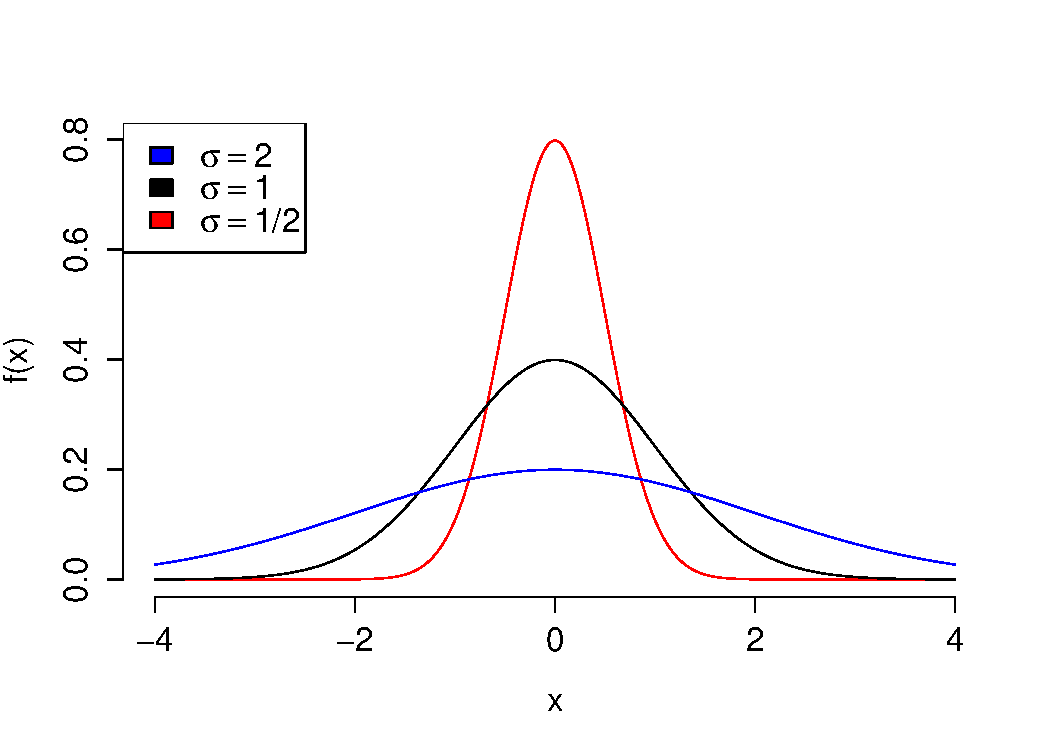
\includegraphics[scale = 0.62]{./images/normal_std_devs}
\end{figure}
\end{frame}

%%%%%%%%%%%%%%%%%%%%%%%%%%%%%%%%%%%%%%%%


\begin{frame}
\frametitle{Linear Function of Normal RV is a Normal RV}


Suppose that $X \sim N(\mu, \sigma^2)$. Then if $a$ and $b$ constants,
$$\boxed{a + bX \sim N(a + b\mu, b^2 \sigma^2)}$$


\begin{block}{Important}
	\begin{itemize}
		\item  Using what know know about expectations of linear functions, no surprise what mean and variance are.
		\item Surprise is that the linear combination is \emph{\alert{normal}}
		\item Linear trans.\ does not preserve, e.g.,  Bernoulli or Binomial.
	\end{itemize}
\end{block}

\end{frame}

%%%%%%%%%%%%%%%%%%%%%%%%%%%%%%%%%%%%%%%%
\begin{frame}
\frametitle{Example \hfill 
\includegraphics[scale = 0.05]{./images/clicker}}
Suppose $X \sim N(\mu, \sigma^2)$ and let $Z = (X -\mu)/\sigma$. What is the distribution of $Z$?

\begin{enumerate}[(a)]
	\item $N(\mu, \sigma^2)$
	\item $N(\mu, \sigma)$
	\item $N(0, \sigma^2)$
	\item  $N(0, \sigma)$
	\item $N(0,1)$
\end{enumerate}
\end{frame}



%%%%%%%%%%%%%%%%%%%%%%%%%%%%%%%%%%%%%%%%
\begin{frame}
\begin{figure}
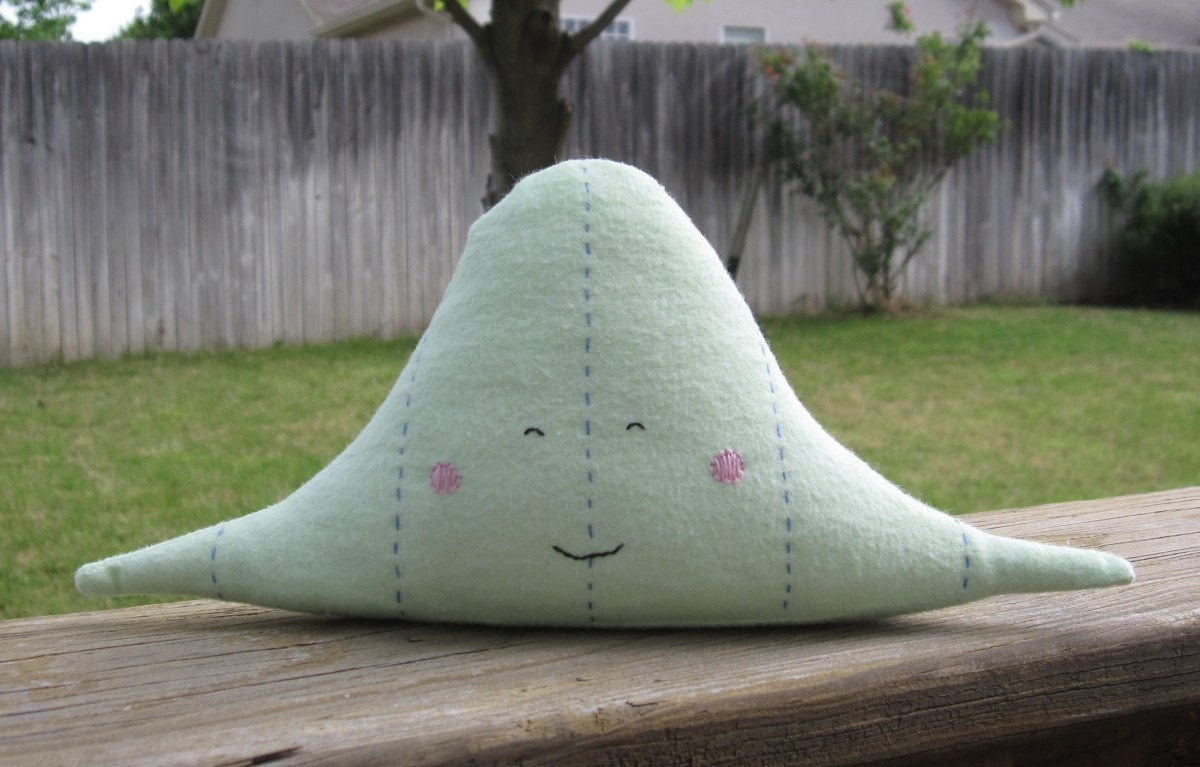
\includegraphics[scale = 0.2]{./images/normal_etsy1}
\caption{Standard Normal Distribution (PDF)}
\end{figure}
\end{frame}

%%%%%%%%%%%%%%%%%%%%%%%%%%%%%%%%%%%%%%%%
\begin{frame}
\frametitle{Standard Normal Distribution: $N(0,1)$}
\begin{figure}
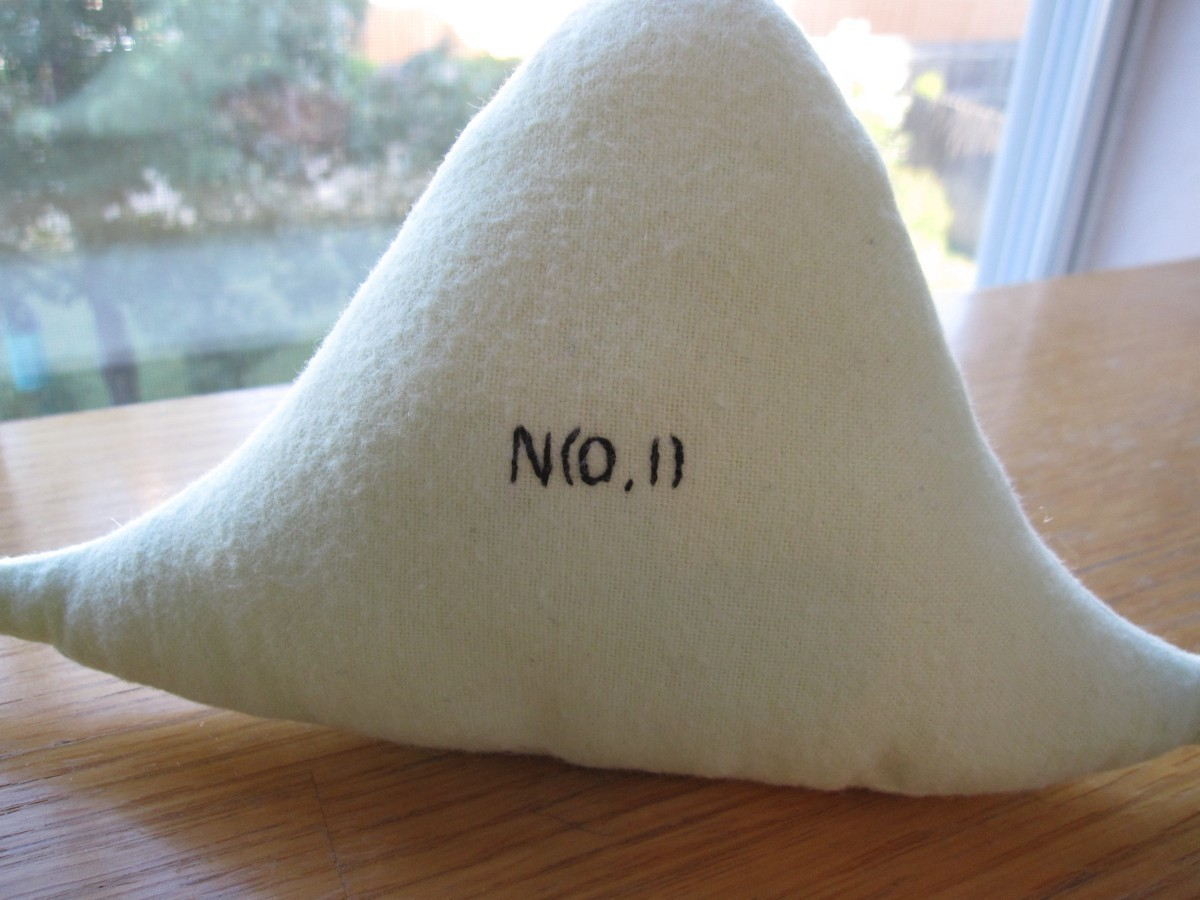
\includegraphics[scale = 0.2]{./images/normal_etsy2}
\end{figure}
\end{frame}
%%%%%%%%%%%%%%%%%%%%%%%%%%%%%%%%%%%%%%%%
\begin{frame}
\frametitle{Standard Normal Distribution: $N(0,1)$}
Mean = 0, Variance = Standard Deviation = 1
	$$f(x) = \frac{1}{\sqrt{2\pi}} e^{-x^2/2}$$

Special symbol for Standard Normal CDF (no closed form):
	$$\Phi(x_0) = \int_{-\infty}^{x_0}\frac{1}{\sqrt{2\pi}} e^{-x^2/2}\; dx $$
	
R Command: $\Phi(x_0) =$\texttt{pnorm()}
\end{frame}



%%%%%%%%%%%%%%%%%%%%%%%%%%%%%%%%%%%%%%%%
%\begin{frame}
%\begin{figure}
%
\includegraphics[scale = 0.2]{./images/normal_etsy_pumpkin}
%\caption{Standard Normal PDF -- Halloween Edition}
%\end{figure}
%\end{frame}
%%%%%%%%%%%%%%%%%%%%%%%%%%%%%%%%%%%%%%%%
%\begin{frame}
%\begin{figure}
%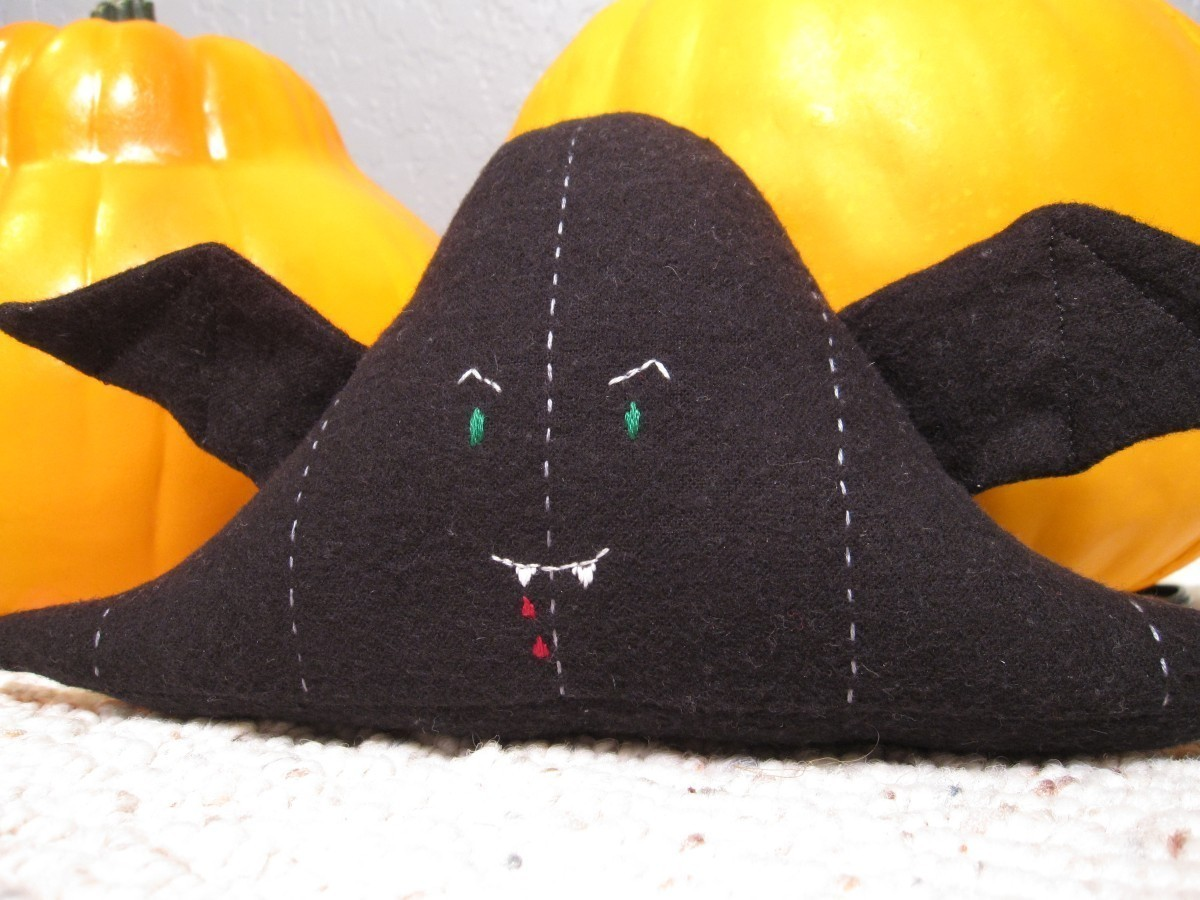
\includegraphics[scale = 0.2]{./images/normal_etsy_bat}
%\caption{Standard Normal PDF -- Alternate Halloween Edition}
%\end{figure}
%\end{frame}
%%%%%%%%%%%%%%%%%%%%%%%%%%%%%%%%%%%%%%%%
\begin{frame}
\frametitle{Where does the Empirical Rule come from?}

\begin{block}{Empirical Rule}
Approximately 68\% of observations within $\mu\pm \sigma$\\
Approximately 95\% of observations within $\mu\pm 2 \sigma$\\
Nearly all observations within $\mu\pm 3 \sigma$\\
\end{block}
\end{frame}

%%%%%%%%%%%%%%%%%%%%%%%%%%%%%%%%%%%%%%%%

\begin{frame}
\frametitle{Middle 68\% of $N(0,1) \Rightarrow$ approx.\ $(-1,1)$}
\begin{figure}
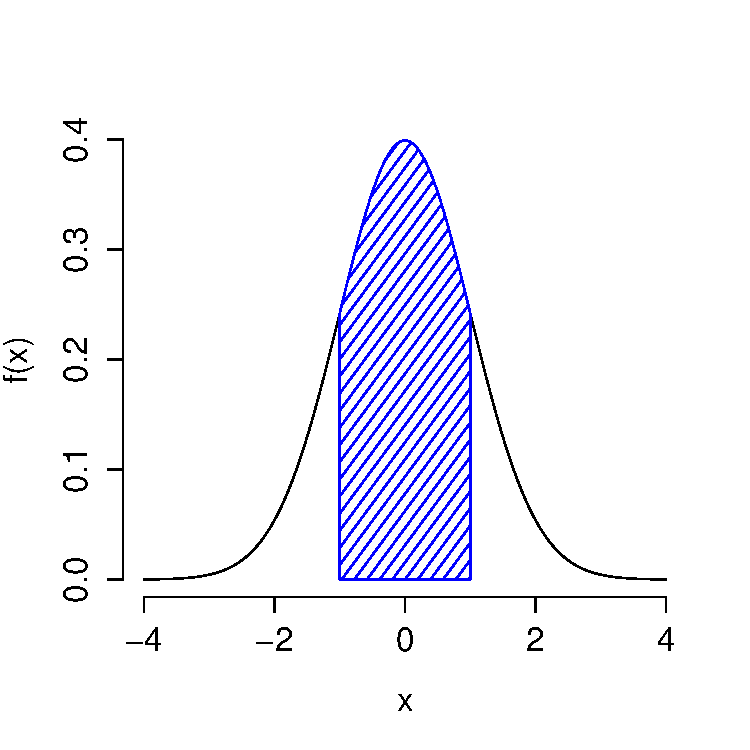
\includegraphics[scale = 0.65]{./images/normal_middle68}
\end{figure}
\end{frame}

%%%%%%%%%%%%%%%%%%%%%%%%%%%%%%%%%%%%%%%%

\begin{frame}
\frametitle{Middle 95\% of $N(0,1)\Rightarrow$ approx.\ $(-2,2)$}

\begin{figure}
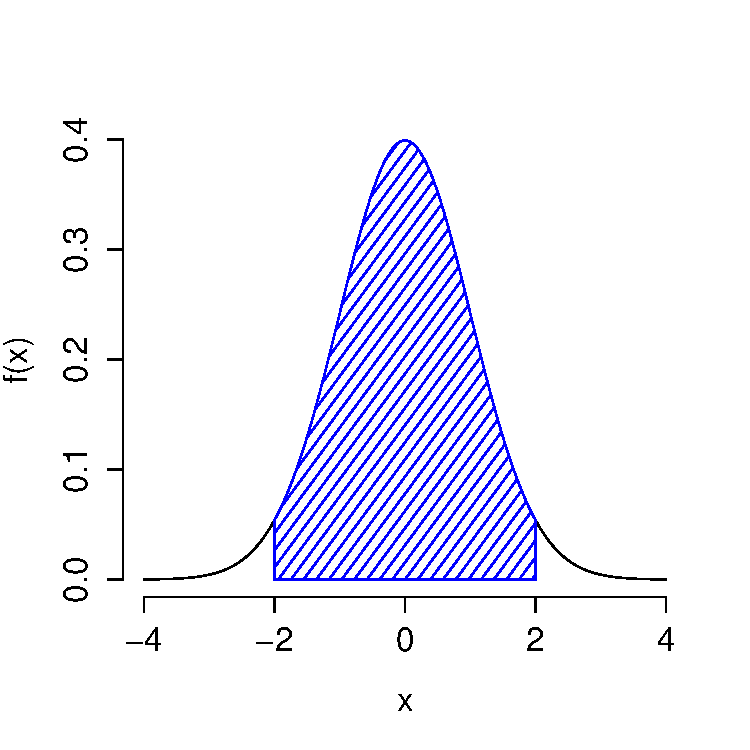
\includegraphics[scale = 0.65]{./images/normal_middle95}
\caption{PDF for t-Distribution}
\end{figure}
\end{frame}
%%%%%%%%%%%%%%%%%%%%%%%%%%%%%%%%%%%%%%%%
\begin{frame}
\frametitle{More Formally...}
$$\int_{-1}^1 \frac{1}{\sqrt{2\pi}} e^{-x^2/2}\; dx  \approx 0.68$$
\vspace{2em}
$$\int_{-2}^2 \frac{1}{\sqrt{2\pi}} e^{-x^2/2}\; dx  \approx 0.95$$
\begin{alertblock}{But how do we know this?}\end{alertblock}
\end{frame}
%%%%%%%%%%%%%%%%%%%%%%%%%%%%%%%%%%%%%%%%

\begin{frame}
\frametitle{$\Phi(1) =$\texttt{pnorm(1)}$\approx 0.84$}

\begin{figure}
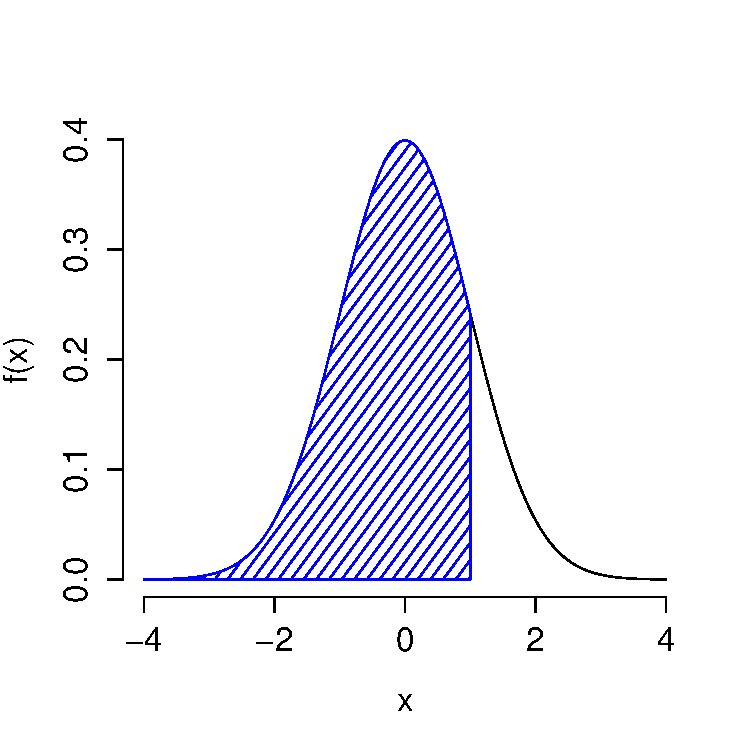
\includegraphics[scale = 0.65]{./images/middle68_1}
\end{figure}
\end{frame}
%%%%%%%%%%%%%%%%%%%%%%%%%%%%%%%%%%%%%%%%
\begin{frame}
\frametitle{$\Phi(1) - \Phi(-1) =$\texttt{pnorm(1) - pnorm(-1)}$\approx 0.84 - 0.16$}
\begin{figure}
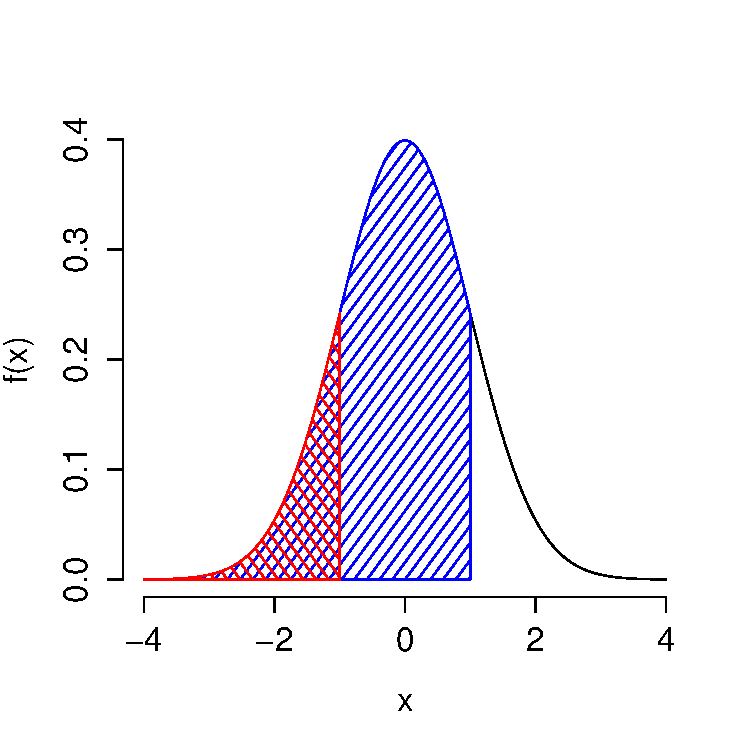
\includegraphics[scale = 0.65]{./images/middle68_2}
\end{figure}
\end{frame}
%%%%%%%%%%%%%%%%%%%%%%%%%%%%%%%%%%%%%%%%
\begin{frame}
\frametitle{$\Phi(1) - \Phi(-1) =$\texttt{pnorm(1) - pnorm(-1)}$\approx 0.68$}
\begin{figure}
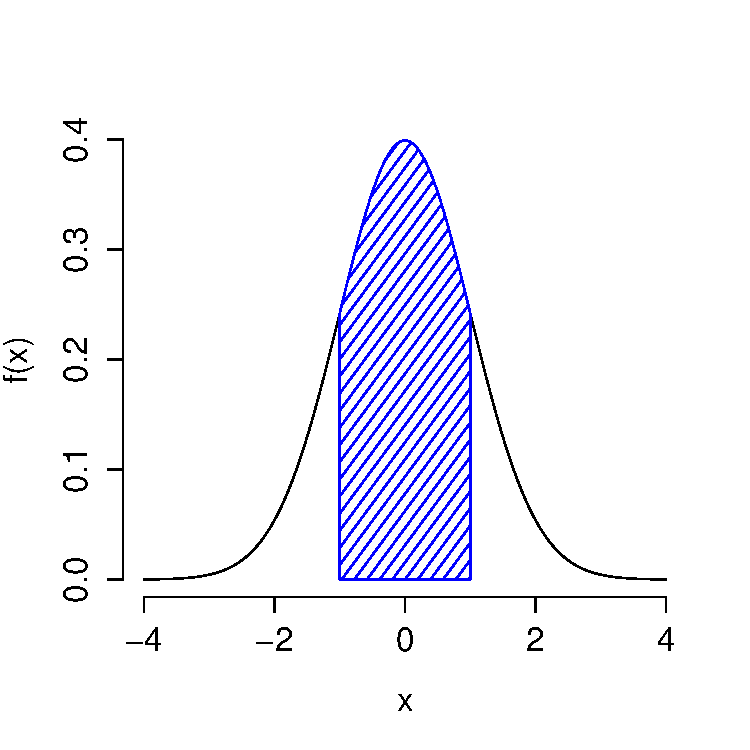
\includegraphics[scale = 0.65]{./images/middle68_3}
\end{figure}
\end{frame}
%%%%%%%%%%%%%%%%%%%%%%%%%%%%%%%%%%%%%%%%
\begin{frame}
\frametitle{Suppose $X \sim N(0,1)$}
\begin{eqnarray*}
	P(-2 \leq X \leq 2) &=& \Phi(2) - \Phi(-2) \\
		&=& \mbox{\texttt{pnorm(2) - pnorm(-2)}}\\
		&\approx& 0.95
\end{eqnarray*}
\pause
\begin{eqnarray*}
	P(-3 \leq X \leq 3) &=& \Phi(3) - \Phi(-3) \\
		&=& \mbox{\texttt{pnorm(3) - pnorm(-3)}}\\
		&\approx& 1
\end{eqnarray*}

\end{frame}
%%%%%%%%%%%%%%%%%%%%%%%%%%%%%%%%%%%%%%%%
%%%%%%%%%%%%%%%%%%%%%%%%%%%%%%%%%%%%%%%%
\begin{frame}
\frametitle{What if $X \sim N(\mu, \sigma^2)$?}
\begin{eqnarray*}
	P(X \leq a) &=& \pause P(X - \mu \leq a - \mu)\\\\
		&=& \pause P\left( \frac{X-\mu}{\sigma} \leq \frac{a - \mu}{\sigma} \right)\\\\
		&=&\pause  P\left(Z \leq  \frac{a - \mu}{\sigma}\right)
\end{eqnarray*}
Where $Z$ is a standard normal random variable, i.e.\ $N(0,1)$.
\end{frame}


%%%%%%%%%%%%%%%%%%%%%%%%%%%%%%%%%%%%%%%%
\begin{frame}
\frametitle{
\includegraphics[scale = 0.05]{./images/clicker}}
Which of these equals $P\left(Z \leq (a-\mu)/\sigma\right)$ if $Z\sim N(0,1)$?
	\begin{enumerate}[(a)]
		\item $\Phi(a)$
		\item $1 - \Phi(a)$
		\item $\Phi(a)/\sigma - \mu$
		\item $\Phi\left(\frac{a - \mu}{\sigma}  \right)$
		\item None of the above.
	\end{enumerate}
\end{frame}
%%%%%%%%%%%%%%%%%%%%%%%%%%%%%%%%%%%%%%%%

\begin{frame}
\frametitle{What if $X \sim N(\mu, \sigma^2)$?}
\begin{eqnarray*}
	P(X \leq a) &=&\ P(X - \mu \leq a - \mu)\\\\
		&=& P\left( \frac{X-\mu}{\sigma} \leq \frac{a - \mu}{\sigma} \right)\\\\
		&=& P\left(Z \leq  \frac{a - \mu}{\sigma}\right)\\
		&=&\alert{\Phi\left(\frac{a - \mu}{\sigma}  \right)}\\
		&=&\alert{ \mbox{\texttt{pnorm}}((a-\mu)/\sigma)}
\end{eqnarray*}
Where $Z$ is a standard normal random variable, i.e.\ $N(0,1)$.
\end{frame}


%%%%%%%%%%%%%%%%%%%%%%%%%%%%%%%%%%%%%%%%
\begin{frame}
\frametitle{Suppose $X \sim N(\mu, \sigma^2)$ \hfill 
\includegraphics[scale = 0.05]{./images/clicker}}
Which of these is $P(X \geq b)$?
\begin{enumerate}[(a)]
	\item $\Phi(b)$
	\item $1 - \Phi\left( \frac{b - \mu}{\sigma} \right)$
	\item $1 - \Phi(b)$
	\item $1 - \left(\Phi(b)/\sigma - \mu\right)$
\end{enumerate}

\end{frame}
\begin{frame}
\frametitle{Suppose $X \sim N(\mu, \sigma^2)$}
\begin{eqnarray*}
	P(X \geq b) &=&\pause 1 - P(X\leq b) =\pause 1 - P\left( \frac{X-\mu}{\sigma} \leq \frac{b-\mu}{\sigma} \right) \\ \\
	&=&\pause 1 - P\left( Z \leq \frac{b-\mu}{\sigma} \right) = 1 - \Phi\left( \frac{b-\mu}{\sigma} \right)\\ \\
	&=&\pause 1 -\mbox{\texttt{pnorm}}((b-\mu)/\sigma)
\end{eqnarray*}
Where $Z$ is a standard normal random variable.
\end{frame}
%%%%%%%%%%%%%%%%%%%%%%%%%%%%%%%%%%%%%%%%
\begin{frame}
\frametitle{Suppose $X \sim N(\mu, \sigma^2)$}


\begin{eqnarray*}
	P(a \leq X \leq b) &=& \pause P\left( \frac{a - \mu}{\sigma} \leq \frac{X - \mu}{\sigma} \leq \frac{b-\mu}{\sigma} \right)\\ \\ 
	&=& \pause P\left( \frac{a - \mu}{\sigma} \leq Z \leq \frac{b-\mu}{\sigma} \right)\\ \\ 
	&=& \pause \Phi\left( \frac{b-\mu}{\sigma}\right) - \Phi\left( \frac{a - \mu}{\sigma}\right)\\ \\
	&=&\pause \mbox{\texttt{pnorm}}((b-\mu)/\sigma) -  \mbox{\texttt{pnorm}}((a-\mu)/\sigma)
\end{eqnarray*}
Where $Z$ is a standard normal random variable.
\end{frame}
%%%%%%%%%%%%%%%%%%%%%%%%%%%%%%%%%%%%%%%%
\begin{frame}
\frametitle{Suppose $X \sim N(\mu, \sigma^2)$\hfill 
\includegraphics[scale = 0.05]{./images/clicker}}
What is $P(\mu - \sigma \leq X \leq \mu + \sigma)$?
\end{frame}

%%%%%%%%%%%%%%%%%%%%%%%%%%%%%%%%%%%%%%%%
\begin{frame}
\frametitle{Suppose $X \sim N(\mu, \sigma^2)$}

\begin{eqnarray*}
P(\mu - \sigma \leq X \leq \mu + \sigma) &=& P\left( -1 \leq \frac{X-\mu}{\sigma} \leq 1\right)\\ \\
	&=& P\left( -1 \leq Z \leq 1\right)\\
	&=& \Phi(1) - \Phi(-1)\\
	&=& \mbox{\texttt{pnorm(1)}} -  \mbox{\texttt{pnorm(-1)}}\\
	&\approx& 0.68
\end{eqnarray*}
\end{frame}

%%%%%%%%%%%%%%%%%%%%%%%%%%%%%%%%%%%%%%%%

\begin{frame}
\frametitle{Suppose $X \sim N(\mu, \sigma^2)$\hfill 
\includegraphics[scale = 0.05]{./images/clicker}}
What is $P(\mu - 2\sigma \leq X \leq \mu + 2\sigma)$?
\end{frame}

%%%%%%%%%%%%%%%%%%%%%%%%%%%%%%%%%%%%%%%%
\begin{frame}
\frametitle{Suppose $X \sim N(\mu, \sigma^2)$}

\begin{eqnarray*}
P(\mu - 2\sigma \leq X \leq \mu + 2\sigma) &=& P\left( -2 \leq \frac{X-\mu}{\sigma} \leq 2\right)\\ \\
	&=& P\left( -2 \leq Z \leq 2\right)\\
	&=& \Phi(2) - \Phi(-2)\\
	&=& \mbox{\texttt{pnorm(2)}} -  \mbox{\texttt{pnorm(-2)}}\\
	&\approx& 0.95
\end{eqnarray*}
\end{frame}


%%%%%%%%%%%%%%%%%%%%%%%%%%%%%%%%%%%%%%%%

\begin{frame}
\frametitle{Percentiles/Quantiles for Continuous RVs}
\begin{block}{Quantile Function $Q(p)$ is the inverse of CDF $F(x_0)$}
Plug in a probability $p$, get out the value of $x_0$ such that $F(x_0)=p$
\end{block}
$$Q(p) = F^{-1}(p)$$

In other words:
	$$Q(p) = \mbox{the value of } x_0 \mbox{ such that } \int_{-\infty}^{x_0} f(x) \; dx = p$$
	
\begin{alertblock}{Inverse exists as long as $F(x_0)$ is \emph{strictly increasing}.} \end{alertblock}	
	
\end{frame}
%%%%%%%%%%%%%%%%%%%%%%%%%%%%%%%%%%%%%%%%
\begin{frame}
\frametitle{Example: Median}
The median of a continuous random variable is $Q(0.5)$, i.e.\ the value of $x_0$ such that 
	$$\int_{-\infty}^{x_0} f(x)\; dx = 1/2$$
\end{frame}
%%%%%%%%%%%%%%%%%%%%%%%%%%%%%%%%%%%%%%%%
\begin{frame}
\frametitle{What is the median of a standard normal RV?\hfill 
\includegraphics[scale = 0.05]{./images/clicker}}
\pause
By symmetry, $Q(0.5) = 0$. R command: \texttt{qnorm()}
\begin{center}
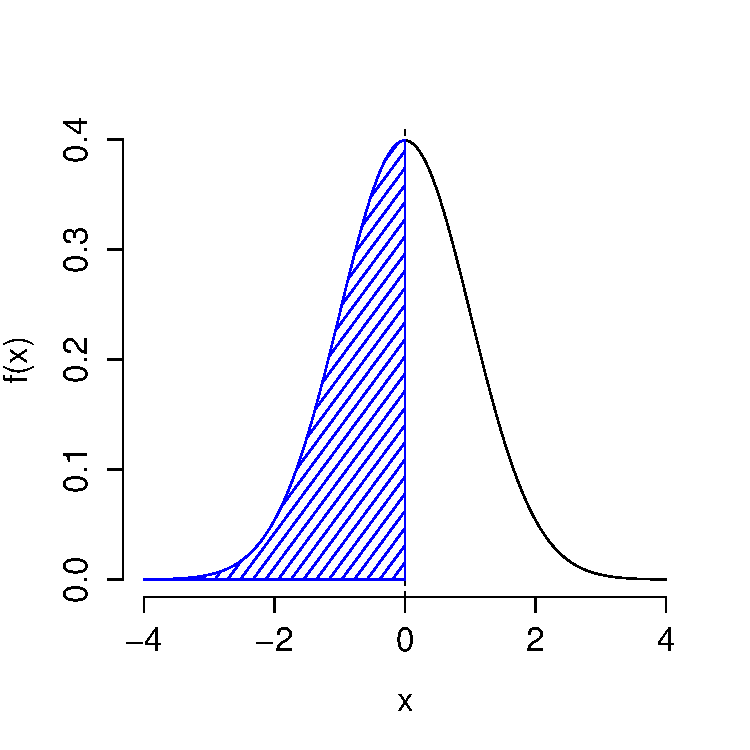
\includegraphics[scale = 0.6]{./images/normal_median}
\end{center}
\end{frame}
%%%%%%%%%%%%%%%%%%%%%%%%%%%%%%%%%%%%%%%%
\begin{frame}
\frametitle{90th Percentile of a Standard Normal}
\texttt{qnorm(0.9)}$\approx 1.28$
\begin{center}
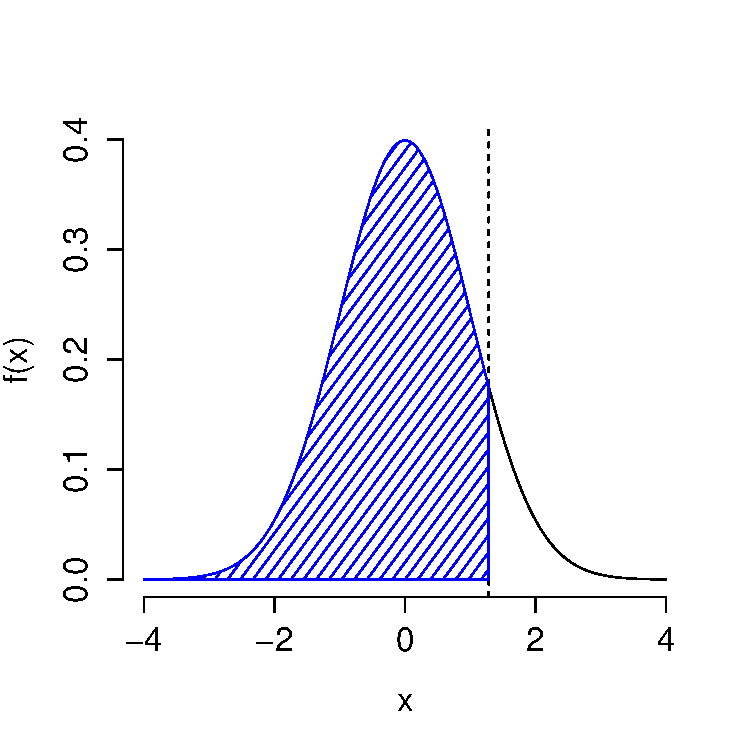
\includegraphics[scale = 0.6]{./images/normal90}
\end{center}
\end{frame}
%%%%%%%%%%%%%%%%%%%%%%%%%%%%%%%%%%%%%%%%

\begin{frame}
\frametitle{Using Quantile Function to find Symmetric Intervals}
Suppose $X$ is a standard normal RV. What is the value of $c$ such that $P(-c \leq X\leq c ) = 0.5$?
\begin{center}
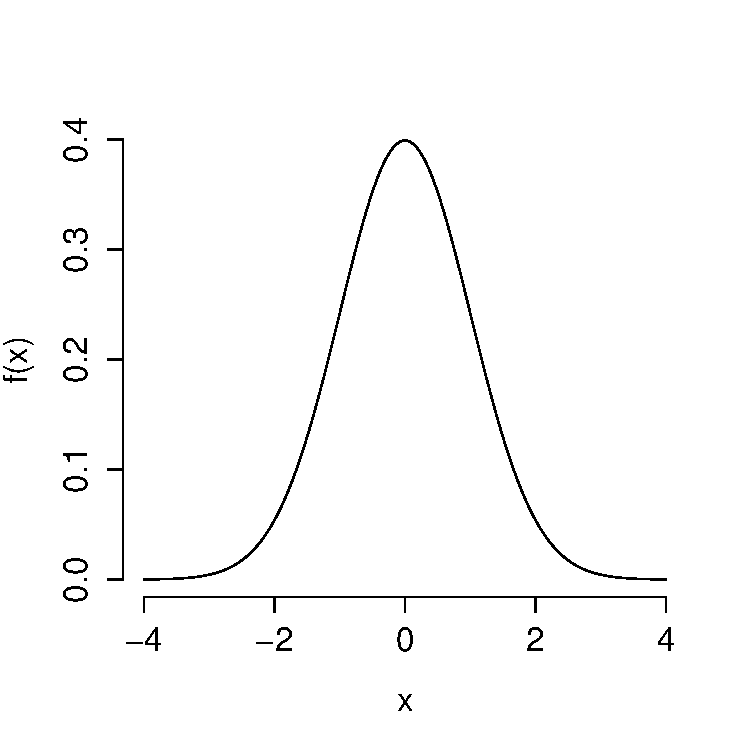
\includegraphics[scale = 0.55]{./images/tail1}
\end{center}
\end{frame}

%%%%%%%%%%%%%%%%%%%%%%%%%%%%%%%%%%%%%%%%
\begin{frame}
\frametitle{\texttt{qnorm(0.75)}$\approx 0.67$}
Suppose $X$ is a standard normal RV. What is the value of $c$ such that $P(-c \leq X\leq c ) = 0.5$?
\begin{center}
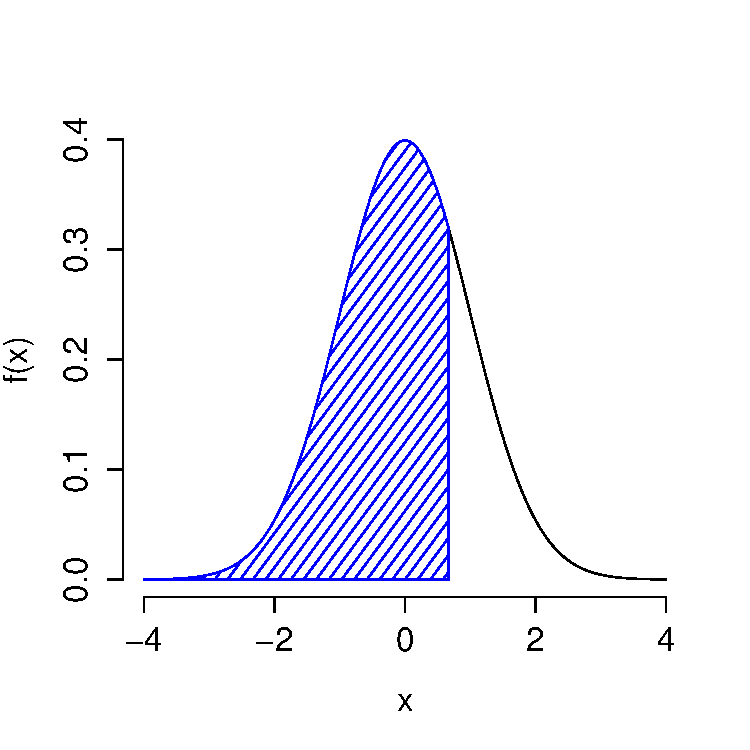
\includegraphics[scale = 0.55]{./images/tail2}
\end{center}
\end{frame}

%%%%%%%%%%%%%%%%%%%%%%%%%%%%%%%%%%%%%%%%
\begin{frame}
\frametitle{\texttt{qnorm(0.75)}$\approx 0.67$}
Suppose $X$ is a standard normal RV. What is the value of $c$ such that $P(-c \leq X\leq c ) = 0.5$?
\begin{center}
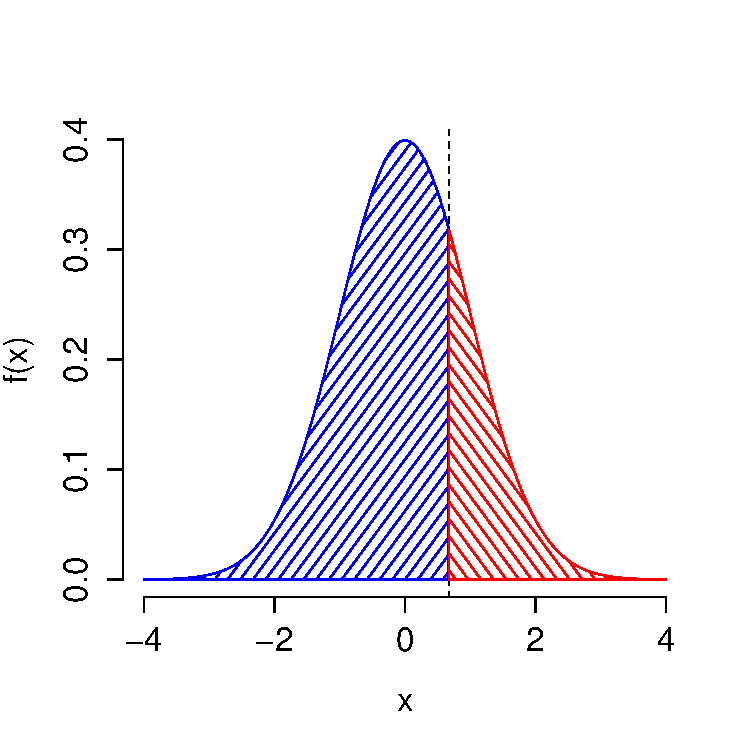
\includegraphics[scale = 0.55]{./images/tail3}
\end{center}
\end{frame}

%%%%%%%%%%%%%%%%%%%%%%%%%%%%%%%%%%%%%%%%

\begin{frame}
\frametitle{\texttt{pnorm(0.67)-pnorm(-0.67)}$\approx$?}
Suppose $X$ is a standard normal RV. What is the value of $c$ such that $P(-c \leq X\leq c ) = 0.5$?
\begin{center}
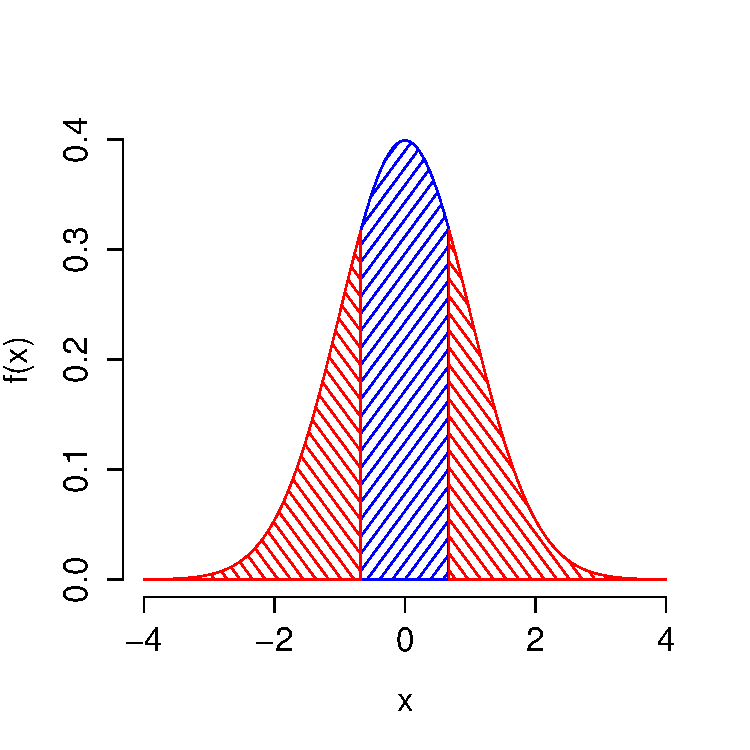
\includegraphics[scale = 0.55]{./images/tail4}
\end{center}
\end{frame}

%%%%%%%%%%%%%%%%%%%%%%%%%%%%%%%%%%%%%%%%


\begin{frame}
\frametitle{\texttt{pnorm(0.67)-pnorm(-0.67)}$\approx 0.5$}
Suppose $X$ is a standard normal RV. What is the value of $c$ such that $P(-c \leq X\leq c ) = 0.5$?
\begin{center}
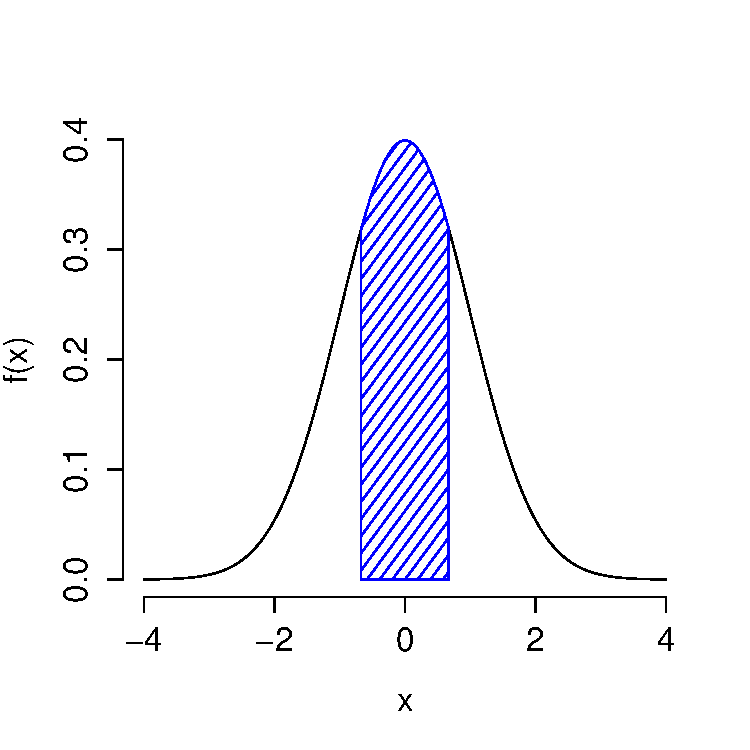
\includegraphics[scale = 0.55]{./images/tail5}
\end{center}
\end{frame}
%%%%%%%%%%%%%%%%%%%%%%%%%%%%%%%%%%%%%%%%
\begin{frame}
\frametitle{68\% Central Interval for Standard Normal \hfill 
\includegraphics[scale = 0.05]{./images/clicker}}

Suppose $X$ is a standard normal random variable. What value of $c$ ensures that $P(-c \leq X \leq c) \approx 0.68$?

\end{frame}


%%%%%%%%%%%%%%%%%%%%%%%%%%%%%%%%%%%%%%%%
\begin{frame}
\frametitle{95\% Central Interval for Standard Normal \hfill 
\includegraphics[scale = 0.05]{./images/clicker}}

Suppose $X$ is a standard normal random variable. What value of $c$ ensures that $P(-c \leq X \leq c) \approx \alert{0.95}$?

\end{frame}


%%%%%%%%%%%%%%%%%%%%%%%%%%%%%%%%%%%%%%%%

\begin{frame}
\frametitle{R Commands for \emph{Arbitrary} Normal Distributions}
Let $X \sim N(\mu, \sigma^2)$ . Then we can use R to evaluate the CDF and Quantile function of $X$ as follows:
\vspace{1em}
\begin{table}
\centering
\fbox{\begin{tabular}{ll}
CDF $F(x)$&\texttt{pnorm(x, mean = $\mu$,  sd = $\sigma$)}\\
Quantile Function $Q(p)$ & \texttt{qnorm(p, mean = $\mu$,  sd = $\sigma$)}\\
\end{tabular}}
\end{table}
\vspace{1em}
\alert{Notice that this means you don't have to transform $X$ to a standard normal in order to find areas under its pdf using R.}
\end{frame}
%%%%%%%%%%%%%%%%%%%%%%%%%%%%%%%%%%%%%%%%
\begin{frame}
\frametitle{Example from Homework: $X \sim N(0,16)$}

One Way:
			\begin{eqnarray*}
				P(X \geq 10) &=&  1 - P(X \leq 10) = 1 - P(X /4\leq 10/4)\\
				&=& 1 - P(Z\leq 2.5) =   1 - \Phi(2.5) =  1 - \mbox{\texttt{pnorm(2.5)}}\\ 
				&\approx& 0.006
			\end{eqnarray*}
\pause
An Easier Way:
	\begin{eqnarray*}
	P(X \geq 10) &=& 1 - P(X \leq 10)\\ 
	&=&  1 - \texttt{pnorm(10, mean = 0, sd = 4)} \\ 
	&\approx& 0.006
	\end{eqnarray*}
\end{frame}
%%%%%%%%%%%%%%%%%%%%%%%%%%%%%%%%%%%%%%%%
\begin{frame}
Suppose $X$ has mean $\mu_x$ variance $\sigma_x^2$ and is independent of $Y$, which has mean $\mu_y$ variance $\sigma_y^2$. Let $a,b$ be constants.
\vspace{2em}

\begin{block}{What is $E[aX + bY]$?}
\pause
$E[aX + bY]=a E[X] + b E[Y] = \alert{a\mu_x + b\mu_y}$
\end{block}
\vspace{1em}

\begin{block}{What is $Var(aX + bY)$?}
\pause
$Var(aX + bY) = a^2 Var(X) + b^2 Var(Y) = \alert{a^2 \sigma_x^2 + b^2 \sigma_y^2}$
\\\alert{By independence.}
\end{block}

\end{frame}
%%%%%%%%%%%%%%%%%%%%%%%%%%%%%%%%%%%%%%%%
\begin{frame}
Now suppose $X \sim N(\mu_x, \sigma^2_x)$ independent of $Y \sim N(\mu_y, \sigma^2_y)$. Let $a,b$ be constants.
\vspace{2em}

\begin{block}{What is $E[aX + bY]$?}
\pause
$E[aX + bY]=a E[X] + b E[Y] = \alert{a\mu_x + b\mu_y}$
\end{block}
\vspace{1em}

\begin{block}{What is $Var(aX + bY)$?}
\pause
$Var(aX + bY) = a^2 Var(X) + b^2 Var(Y) = \alert{a^2 \sigma_x^2 + b^2 \sigma_y^2}$
\\\alert{By independence.}
\end{block}
\end{frame}
%%%%%%%%%%%%%%%%%%%%%%%%%%%%%%%%%%%%%%%%
\begin{frame}
\frametitle{Here's the Surprising Thing:}
\alert{If $X$ and $Y$ are independent Normal Random Variables and $a,b$ are constants, then $aX + bY$ is \emph{also} a Normal Random Variable!}
\end{frame}
%%%%%%%%%%%%%%%%%%%%%%%%%%%%%%%%%%%%%%%%
\begin{frame}
\frametitle{Linear Combinations of Independent Normals}
Let $X \sim N(\mu_x, \sigma^2_x)$ independent of $Y \sim N(\mu_y, \sigma^2_y)$. Then if $a,b,c$ are constants:

$$\boxed{aX + bY +c \sim N(a\mu_x + b\mu_y + c, a^2 \sigma_x^2 + b^2 \sigma_y^2)}$$



\begin{block}{Important}
	\begin{itemize}
		\item Result assumes independence
		\item Particular to Normal Distribution
		\item Extends to more than two Normal RVs
	\end{itemize}
\end{block}

\end{frame}
%%%%%%%%%%%%%%%%%%%%%%%%%%%%%%%%%%%%%%%%
\begin{frame}
\frametitle{Suppose $X_1, X_2, \sim \mbox{iid } N(\mu, \sigma^2)$ \hfill 
\includegraphics[scale = 0.05]{./images/clicker}}

Let $\bar{X} = (X_1 + X_2)/2$. What is the distribution of $\bar{X}$?
\begin{enumerate}[(a)]
\item $N(\mu, \sigma^2/2)$
\item $N(0,1)$
\item $N(\mu, \sigma^2)$
\item $N(\mu, 2\sigma^2)$
\item $N(2\mu, 2\sigma^2)$
\end{enumerate}

\end{frame}
%%%%%%%%%%%%%%%%%%%%%%%%%%%%%%%%%%%%%%%%

\end{document}
